\documentclass[11pt]{article}
\usepackage[margin=2cm]{geometry}
\usepackage{microtype}
\usepackage{float}
\usepackage{graphicx}
\usepackage{natbib}
\usepackage{amsmath}

\title{Advanced Techniques in Macroeconomics\\Research Proposal\\Inflation Expectations at the Zero Lower Bound}
\author{Damian Romero}
\date{November 22, 2016}

\begin{document}
	
\maketitle

\section*{Motivation} 

United States example of the disparity between inflation expectations and current inflation, specially during the period of zero lower bound (ZLB). In Figure \ref{fig:motivation}, I present inflation measured as the percent change 12 months ago in the Consumer Price Index for all Urban Consumers (seasonally adjusted) taken from FRED database, inflation expectations taken from the Survey of Consumers by the University of Michigan, and inflation expectations from professional forecasters taken from Consensus Forecast. The first measure of expectation corresponds to the median expected price change in the next 12 months, while the second measure considers expectations for next year. The three measures are highly correlated both pre and during the ZLB period. However, during the latter period we observe a clear difference between household expectations and the actual measure.
%Could be interesting to present other cases in which the ZLB has been reached and see what happens there. If supports the idea, keep it. Else, drop it.

\begin{figure}[H]
	\centering
	\caption{Inflation and inflation expectations in the US}\label{fig:motivation}
	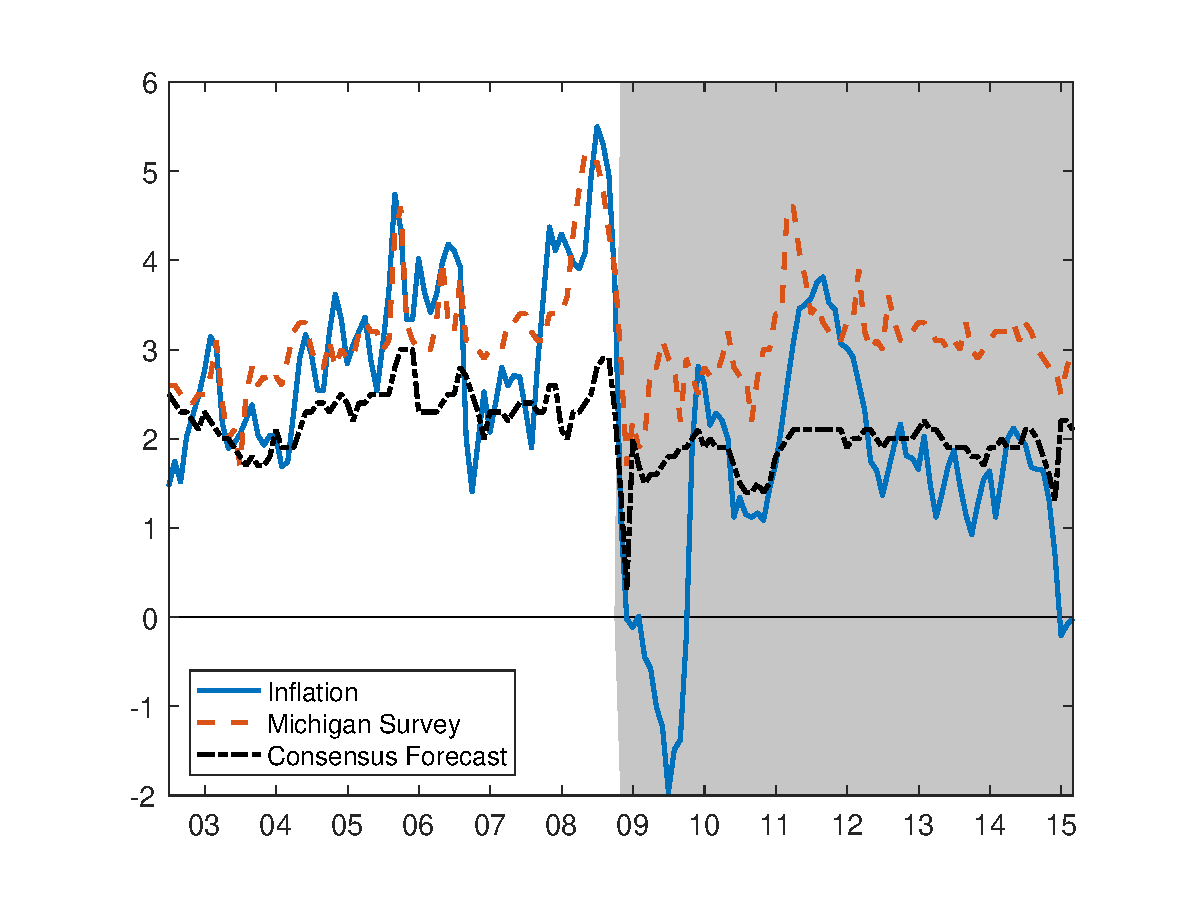
\includegraphics[scale=0.7]{motivation}
\end{figure}

\section*{Objectives} 

The main objective is to evaluate the properties of the standard New Keynesian model (NKM) regarding the periods of ZLB. In particular, the goals are (a) characterize inflation expectations in basic NKM that considers as an equilibrium object the ZLB, using global solution methods (mostly in line with \cite{Fernandez-VillaverdeEtAl2015}). Conclude if the model is able to reproduce the empirical patterns or not; (b) incorporate unconventional monetary policies (quantitative easing, forward guidance) into the model and characterize inflation expectations in this context. The prior is that these phenomena should be behind the results, so having these alternative policies would help the economy to recover from the crisis but also keeps the nominal interest rate at the ZLB, making conventional monetary policy ineffective.

\section*{Plan} 

(a) Solve the basic model (a combination of \cite{Fernandez-VillaverdeEtAl2015} and \cite{Gali2015}); (b) obtain policy function for inflation and inflation expectation, analyzing what happens during periods of ZLB; (c) if feasible, incorporate unconventional monetary policies.

\section*{Preview of the model}

We derived the model in Appendix \ref{app:derivation} of this note and here we summarize the main equations.

\subsection*{Equilibrium}

The equilibrium is defined by the sequences $\{Y_t, C_t, N_t, MC_t, F_t, S_t, (W_t/P_t), \Pi_t, \Pi_t^*, \Delta_t, A_t, Z_t\}$ which satisfies:

\begin{enumerate}
\item The first order conditions of the household:

\begin{align}
C_t^{\sigma}N_t^{\varphi}&=\frac{W_t}{P_t}\label{eq1}\\
Q_t&=\beta E_t\left[\left(\frac{C_t}{C_{t+1}}\right)^{\sigma}\frac{P_t}{P_{t+1}}\right]\label{eq2}
\end{align}

\item The first order conditions of the firm:

\begin{align}
F_t&=\left(\frac{\epsilon}{\epsilon-1}\right)S_t\label{eq3}\\
F_t&=\Pi_t^*\left\{\frac{Y_{t}}{C_{t}^{\sigma}}+(\theta\beta)E_t[(\Pi_{t+1}^*)^{-1}(\Pi_{t+1}^{\epsilon-1})F_{t+1}]\right\}\label{eq4}\\
S_t&=(\Pi_t^*)^{\frac{-\alpha\epsilon}{1-\alpha}}\left\{\left(\frac{Y_{t}^{\frac{1}{1-\alpha}}}{C_{t}^{\sigma}}\right)\left(\frac{W_{t}/P_{t}}{(1-\alpha)A_{t}^{\frac{1}{1-\alpha}}}\right)+(\theta\beta)E_t[(\Pi_{t+1}^*)^{\frac{\alpha\epsilon}{1-\alpha}}(\Pi_{t+1})^{\frac{\epsilon}{1-\alpha}}S_{t+1}]\right\}\nonumber\\
MC_t&=\left(\frac{W_t}{(1-\alpha)A_t^{\frac{1}{1-\alpha}}}\right)Y_t^{\frac{\alpha}{1-\alpha}}\nonumber
\end{align}

Note that we could define the real marginal cost dividing by $P_t$. Also, we could multiply and divide by $Y_t^{\frac{1}{1-\alpha}}$. Re-arranging, we have the final expression for real marginal costs:

\begin{align}
RMC_t=\left[\left(\frac{W_t/P_t}{(1-\alpha)A_t^{\frac{1}{1-\alpha}}}\right)Y_t^{\frac{1}{1-\alpha}}\right]\frac{1}{Y_t}\label{eq5}
\end{align}

With this definition, we could re-writte expression $S_t$:

\begin{align}
S_t&=(\Pi_t^*)^{\frac{-\alpha\epsilon}{1-\alpha}}\left\{\frac{RMC_t}{C_t^{\sigma}Y_t}+(\theta\beta)E_t[(\Pi_{t+1}^*)^{\frac{\alpha\epsilon}{1-\alpha}}(\Pi_{t+1})^{\frac{\epsilon}{1-\alpha}}S_{t+1}]\right\}\label{eq6}
\end{align}

\item The monetary policy rule:

\begin{align}
\frac{R_t}{R}=\left(\frac{\Pi_t}{\Pi}\right)^{\phi_{\Pi}}\left(\frac{Y_t}{Y}\right)^{\phi_Y}\label{eq7}
\end{align}

\item The evolution of prices:\footnote{See Appendix \ref{app:recursive_price_disp} for a derivation of the second expression.}

\begin{align}
1&=(1-\theta)(\Pi_t^*)^{1-\epsilon}+\theta(\Pi_t)^{\epsilon-1}\label{eq8}\\
\Delta_t&=(1-\theta)(\Pi_t^*)^{\frac{-\epsilon}{1-\alpha}}+\theta(\Pi_t)^{\frac{\epsilon}{1-\alpha}}\Delta_{t-1}\label{eq9}
\end{align}

\item The market aggregation:

\begin{align}
Y_t&=C_t\label{eq10}\\
Y_t&=\frac{A_tN_t^{1-\alpha}}{\Delta_t^{1-\alpha}}\label{eq11}
\end{align}

\item The exogenous processes:

\begin{align}
\log(A_t)&=\rho_A\log(A_{t-1})+\varepsilon_t^A, \qquad \varepsilon_t^A \sim N(0,\sigma_A)
\label{eq12}\\
\log(Z_t)&=\rho_Z\log(Z_{t-1})+\varepsilon_t^Z, \qquad \varepsilon_t^Z \sim N(0,\sigma_Z)\label{eq13}
\end{align}

\end{enumerate}


%%GATHER{tbib.bib}
\bibliographystyle{agsm}
\bibliography{tbib}

\appendix

\section{Derivation of the model}\label{app:derivation}

\subsection*{Households}

The representative infinite-lived household wants to maximize the present value of its consumption:

\begin{align*}
E_t\sum_{t=0}^{\infty}\beta^tU(C_t,N_t)
\end{align*}

where $N_t$ is the labor offered by the household and $C_t$ is a consumption index defined as:

\begin{align*}
C_t\equiv\left(\int_0^1C_t(i)^{\frac{\epsilon-1}{\epsilon}}di\right)^{\frac{\epsilon}{\epsilon-1}}
\end{align*}

where $i$ is the index of varieties of consumption. 

The period budget constraint is:

\begin{align*}
\int_0^1P_t(i)C_t(i)di+Q_tB_t\leq B_{t-1}+W_tN_t+T_t
\end{align*}

The decision of consumption expenditures among the different goods could be summarized in the set of demand equations:

\begin{align*}
C_t(i)=\left(\frac{P_t(i)}{P_t}\right)^{-\epsilon}C_t
\end{align*}

where $P_t\equiv\left(\int_0^1P_t(i)^{1-\epsilon}di\right)^{\frac{1}{1-\epsilon}}$ is an aggregate price index.\footnote{This demands are obtained from the solution of the expenditure minimization problem, subject to the total expenditure. More formally, the problem is:

\begin{align*}
\min \left(\int_0^1C_t(i)^{\frac{\epsilon-1}{\epsilon}}di\right)^{\frac{\epsilon}{\epsilon-1}}
\intertext{subject to}
\int_0^1P_t(i)C_t(i)di\equiv Z_t
\end{align*}

where $Z_t$ is a given level of expenditure.} Conditional in this optimization, we can re-write the budget constraint as:

\begin{align*}
P_tC_t+Q_tB_t\leq B_{t-1}+W_tN_t+T_t
\end{align*}

Assuming a CES utility function like:

\begin{align*}
U(C_t,N_t)=\frac{C_t^{1-\sigma}}{1-\sigma}-\frac{N_t^{1+\varphi}}{1+\varphi}
\end{align*}

the first order conditions are:

\begin{align*}
C_t^{\sigma}N_t^{\varphi}&=\frac{W_t}{P_t}\\
Q_t&=\beta E_t\left[\left(\frac{C_t}{C_{t+1}}\right)^{\sigma}\frac{P_t}{P_{t+1}}\right]
\end{align*}

where $Q_t$ is the stochastic discount factor.

\subsection*{Firms}

\subsubsection*{Production function}

Given that we have a continuum of varieties of consumption, we also have a continuum of firms producing those. We assume the following technology:

\begin{align*}
Y_t(i)=A_tN_t(i)^{1-\alpha}, \quad \alpha\in[0,1]
\end{align*}

where $A_t$ is the level of technology (assumed to be constant across firms). Given this production function, we know that the total cost of the firm ($CT_t$) is:

\begin{align*}
CT_t=W_t\left(\frac{Y_t}{A_t}\right)^{\frac{1}{1-\alpha}}
\end{align*}

Also, the marginal cost ($MC_t$) is defined as:

\begin{align*}
MC_t\equiv\frac{\partial CT_t}{\partial Y_t} = \left(\frac{W_t}{(1-\alpha)A_t^{\frac{1}{1-\alpha}}}\right)Y_t^{\frac{\alpha}{1-\alpha}}
\end{align*}

\subsubsection*{Price dynamics}

Each period a measure $1-\theta$ of producers reset their prices, while a fraction $\theta$ keep their prices unchanged, so $\theta$ is the degree of price stickiness in the economy. Given this, firms will choose their prices (the optimal price is $P_t^*$) according to maximize the expected value of their profits in the period that prices will be fixed, subject to the sequence of demand constraints derived previously:

\begin{align*}
\max_{P_t^*} \sum_{k=0}^{\infty}\theta^k E_t[Q_{t,t+k}(P_t^*Y_{t+k}-CT_{t+k})] \quad \text{st} \quad C_t(i)=\left(\frac{P_t(i)}{P_t}\right)^{-\epsilon}C_t
\end{align*}

Applying the equilibrium condition that production is equal to consumption in each period (formalized latter) and using the definition of total cost, we can re-writte this problem as:

\begin{align*}
&\max_{P_t^*} \sum_{k=0}^{\infty}\theta^k E_t\left\{Q_{t,t+k}\left[P_t^*\left(\frac{P_t^*}{P_{t+k}}\right)^{-\epsilon}Y_{t+k}-W_{t+k}\left(\frac{\left(\frac{P_t^*}{P_{t+k}}\right)^{-\epsilon}Y_{t+k}}{A_{t+k}}\right)^{\frac{1}{1-\alpha}}\right]\right\}\\
&\max_{P_t^*} \sum_{k=0}^{\infty}\theta^k E_t\left\{Q_{t,t+k}\left[(P_t^*)^{1-\epsilon}(P_{t+k})^{\epsilon}Y_{t+k}-W_{t+k}\left(\frac{(P_{t+k})^{\epsilon}Y_{t+k}}{A_{t+k}}\right)^{\frac{1}{1-\alpha}}(P_t^*)^{\frac{-\epsilon}{1-\alpha}}\right]\right\}
\end{align*}

The first order condition of this problem is:

{\small
\begin{align*}
&\sum_{k=0}^{\infty}\theta^k E_t\left\{Q_{t,t+k}\left[(1-\epsilon)(P_t^*)^{-\epsilon}(P_{t+k})^{\epsilon}Y_{t+k}-\left(\frac{-\epsilon}{1-\alpha}\right)W_{t+k}\left(\frac{(P_{t+k})^{\epsilon}Y_{t+k}}{A_{t+k}}\right)^{\frac{1}{1-\alpha}}(P_t^*)^{\frac{-\epsilon}{1-\alpha}-1}\right]\right\}=0
\end{align*}
}

Dividing both sides by $(1-\epsilon)(P_t^*)^{-1-\epsilon}$

\begin{align*}
&\sum_{k=0}^{\infty}\theta^k E_t\left\{Q_{t,t+k}\left[(P_t^*)(P_{t+k})^{\epsilon}Y_{t+k}-\left(\frac{\epsilon}{\epsilon-1}\right)\left(\frac{W_{t+k}}{1-\alpha}\right)\left(\frac{(P_{t+k})^{\epsilon}Y_{t+k}}{A_{t+k}}\right)^{\frac{1}{1-\alpha}}(P_t^*)^{\frac{-\epsilon}{1-\alpha}+\epsilon}\right]\right\}=0
\end{align*}

Replacing the definition of the stochastic discount factor:

{\footnotesize
\begin{align*}
&\sum_{k=0}^{\infty}(\theta\beta)^k E_t\left\{ \left[\left(\frac{C_t}{C_{t+k}}\right)^{\sigma}\frac{P_t}{P_{t+k}}\right]\left[(P_t^*)(P_{t+k})^{\epsilon}Y_{t+k}-\left(\frac{\epsilon}{\epsilon-1}\right)\left(\frac{W_{t+k}}{1-\alpha}\right)\left(\frac{(P_{t+k})^{\epsilon}Y_{t+k}}{A_{t+k}}\right)^{\frac{1}{1-\alpha}}(P_t^*)^{\frac{-\epsilon}{1-\alpha}+\epsilon}\right]\right\}=0\\
&\sum_{k=0}^{\infty}(\theta\beta)^k E_t\left\{ \left[\left(\frac{1}{C_{t+k}}\right)^{\sigma}\frac{1}{P_{t+k}}\right]\left[(P_t^*)(P_{t+k})^{\epsilon}Y_{t+k}-\left(\frac{\epsilon}{\epsilon-1}\right)\left(\frac{W_{t+k}}{1-\alpha}\right)\left(\frac{(P_{t+k})^{\epsilon}Y_{t+k}}{A_{t+k}}\right)^{\frac{1}{1-\alpha}}(P_t^*)^{\frac{-\epsilon}{1-\alpha}+\epsilon}\right]\right\}=0
\end{align*}
}

Dividing each side of the previous expression by $P_t^{\epsilon}$ and working separately with each side\\

\underline{Left-hand side:}

\begin{align*}
F_t&\equiv\sum_{k=0}^{\infty}(\theta\beta)^k E_t\left\{ \left[\left(\frac{1}{C_{t+k}}\right)^{\sigma}\frac{P_t^{-\epsilon}}{P_{t+k}}\right]\left[(P_t^*)(P_{t+k})^{\epsilon}Y_{t+k}\right]\right\}\\
F_t&\equiv\sum_{k=0}^{\infty}(\theta\beta)^k E_t\left[\left(\frac{Y_{t+k}}{C_{t+k}^{\sigma}}\right)\left(\frac{P_{t+k}}{P_{t}}\right)^{\epsilon-1}\left(\frac{P_t^*}{P_{t}}\right)\right]
\end{align*}

\underline{Right-hand side:}

\begin{align*}
S_t\equiv&\sum_{k=0}^{\infty}(\theta\beta)^k E_t\left\{ \left[\left(\frac{1}{C_{t+k}}\right)^{\sigma}\frac{P_t^{-\epsilon}}{P_{t+k}}\right]\left[\left(\frac{W_{t+k}}{1-\alpha}\right)\left(\frac{(P_{t+k})^{\epsilon}Y_{t+k}}{A_{t+k}}\right)^{\frac{1}{1-\alpha}}(P_t^*)^{\frac{-\epsilon}{1-\alpha}+\epsilon}\right]\right\}\\
S_t\equiv&\sum_{k=0}^{\infty}(\theta\beta)^k E_t\left\{ \left(\frac{Y_{t+k}^{\frac{1}{1-\alpha}}}{C_{t+k}^{\sigma}}\right)\left(\frac{W_{t+k}}{(1-\alpha)A_{t+k}^{\frac{1}{1-\alpha}}}\right)P_t^{-\epsilon}(P_{t+k})^{\frac{\epsilon}{1-\alpha}-1}(P_t^*)^{\frac{-\epsilon}{1-\alpha}+\epsilon}\right\}\\
S_t\equiv&\sum_{k=0}^{\infty}(\theta\beta)^k E_t\left\{ \left(\frac{Y_{t+k}^{\frac{1}{1-\alpha}}}{C_{t+k}^{\sigma}}\right)\left(\frac{W_{t+k}}{(1-\alpha)A_{t+k}^{\frac{1}{1-\alpha}}}\right)\left(\frac{P_{t+k}}{P_t^*}\right)^{\frac{\epsilon}{1-\alpha}}\left(\frac{P_{t}^*}{P_t}\right)^{\epsilon}(P_{t+k}^{-1})\right\}\\
S_t\equiv&\sum_{k=0}^{\infty}(\theta\beta)^k E_t\left\{ \left(\frac{Y_{t+k}^{\frac{1}{1-\alpha}}}{C_{t+k}^{\sigma}}\right)\left(\frac{W_{t+k}/P_{t+k}}{(1-\alpha)A_{t+k}^{\frac{1}{1-\alpha}}}\right)\left(\frac{P_{t+k}}{P_t}\right)^{\frac{\epsilon}{1-\alpha}}\left(\frac{P_{t}^*}{P_t}\right)^{\frac{-\alpha\epsilon}{1-\alpha}}\right\}
\end{align*}

Where the last expression defines real wage ($W_{t+k}/P_{t+k}$).

Combining both expressions we have:

\begin{align*}
F_t=\left(\frac{\epsilon}{\epsilon-1}\right)S_t
\end{align*}

Defining $\Pi^*\equiv P_t^*/P_t$ and $\Pi_{t+k}=P_{t+k}/P_t$, both terms could be written in a recursive way. For $F_t$ we have:

\begin{align*}
F_t&\equiv\sum_{k=0}^{\infty}(\theta\beta)^k E_t\left[\left(\frac{Y_{t+k}}{C_{t+k}^{\sigma}}\right)\left(\frac{P_{t+k}}{P_{t}}\right)^{\epsilon-1}\left(\frac{P_t^*}{P_{t}}\right)\right]\\
F_t&=\Pi_t^*\left\{\frac{Y_{t}}{C_{t}^{\sigma}}+\sum_{k=0}^{\infty}(\theta\beta)^{k+1} E_t\left[\left(\frac{Y_{t+k+1}}{C_{t+k+1}^{\sigma}}\right)\left(\frac{P_{t+k+1}}{P_{t}}\right)^{\epsilon-1}\right]\right\}
\end{align*}

Using the definition of $F_{t+1}$:

\begin{align*}
F_{t+1}&=\sum_{k=0}^{\infty}(\theta\beta)^k E_t\left[\left(\frac{Y_{t+k+1}}{C_{t+k+1}^{\sigma}}\right)\left(\frac{P_{t+k+1}}{P_{t+1}}\right)^{\epsilon-1}\left(\frac{P_{t+1}^*}{P_{t+1}}\right)\right]\\
F_{t+1}&=\Pi_{t+1}^*\sum_{k=0}^{\infty}(\theta\beta)^k E_t\left[\left(\frac{Y_{t+k+1}}{C_{t+k+1}^{\sigma}}\right)\left(\frac{P_{t+k+1}}{P_{t+1}}\right)^{\epsilon-1}\left(\frac{P_{t}}{P_{t}}\right)^{\epsilon-1}\right]\\
F_{t+1}&=\Pi_{t+1}^*\sum_{k=0}^{\infty}(\theta\beta)^k E_t\left[\left(\frac{Y_{t+k+1}}{C_{t+k+1}^{\sigma}}\right)\left(\frac{P_{t+k+1}}{P_{t}}\right)^{\epsilon-1}\left(\frac{P_{t+1}}{P_{t}}\right)^{1-\epsilon}\right]\\
\end{align*}

Combining expressions:

\begin{align*}
F_t&=\Pi_t^*\left\{\frac{Y_{t}}{C_{t}^{\sigma}}+(\theta\beta)E_t[(\Pi_{t+1}^*)^{-1}(\Pi_{t+1}^{\epsilon-1})F_{t+1}]\right\}
\end{align*}

For $S_t$ we have:

\begin{align*}
S_t&\equiv\sum_{k=0}^{\infty}(\theta\beta)^k E_t\left\{ \left(\frac{Y_{t+k}^{\frac{1}{1-\alpha}}}{C_{t+k}^{\sigma}}\right)\left(\frac{W_{t+k}/P_{t+k}}{(1-\alpha)A_{t+k}^{\frac{1}{1-\alpha}}}\right)\left(\frac{P_{t+k}}{P_t}\right)^{\frac{\epsilon}{1-\alpha}}\left(\frac{P_{t}^*}{P_t}\right)^{\frac{-\alpha\epsilon}{1-\alpha}}\right\}\\
\end{align*}

{\scriptsize
\begin{align*}
S_t&=(\Pi_t^*)^{\frac{-\alpha\epsilon}{1-\alpha}}\left\{\left(\frac{Y_{t}^{\frac{1}{1-\alpha}}}{C_{t}^{\sigma}}\right)\left(\frac{W_{t}/P_{t}}{(1-\alpha)A_{t}^{\frac{1}{1-\alpha}}}\right)+\sum_{k=0}^{\infty}(\theta\beta)^{k+1} E_t\left\{ \left(\frac{Y_{t+k+1}^{\frac{1}{1-\alpha}}}{C_{t+k+1}^{\sigma}}\right)\left(\frac{W_{t+k+1}/P_{t+k+1}}{(1-\alpha)A_{t+k+1}^{\frac{1}{1-\alpha}}}\right)\left(\frac{P_{t+k+1}}{P_t}\right)^{\frac{\epsilon}{1-\alpha}}\right\}\right\}
\end{align*}
}

For $S_{t+1}$:

\begin{align*}
S_{t+1}&\equiv\sum_{k=0}^{\infty}(\theta\beta)^k E_t\left\{ \left(\frac{Y_{t+k+1}^{\frac{1}{1-\alpha}}}{C_{t+k+1}^{\sigma}}\right)\left(\frac{W_{t+k+1}/P_{t+k+1}}{(1-\alpha)A_{t+k+1}^{\frac{1}{1-\alpha}}}\right)\left(\frac{P_{t+k+1}}{P_{t+1}}\right)^{\frac{\epsilon}{1-\alpha}}\left(\frac{P_{t+1}^*}{P_{t+1}}\right)^{\frac{-\alpha\epsilon}{1-\alpha}}\right\}\\
S_{t+1}&=(\Pi_{t+1}^*)^{\frac{-\alpha\epsilon}{1-\alpha}}\sum_{k=0}^{\infty}(\theta\beta)^k E_t\left\{ \left(\frac{Y_{t+k+1}^{\frac{1}{1-\alpha}}}{C_{t+k+1}^{\sigma}}\right)\left(\frac{W_{t+k+1}/P_{t+k+1}}{(1-\alpha)A_{t+k+1}^{\frac{1}{1-\alpha}}}\right)\left(\frac{P_{t+k+1}}{P_{t+1}}\right)^{\frac{\epsilon}{1-\alpha}}\left(\frac{P_{t}}{P_{t}}\right)^{\frac{\epsilon}{1-\alpha}}\right\}\\
S_{t+1}&=(\Pi_{t+1}^*)^{\frac{-\alpha\epsilon}{1-\alpha}}\sum_{k=0}^{\infty}(\theta\beta)^k E_t\left\{ \left(\frac{Y_{t+k+1}^{\frac{1}{1-\alpha}}}{C_{t+k+1}^{\sigma}}\right)\left(\frac{W_{t+k+1}/P_{t+k+1}}{(1-\alpha)A_{t+k+1}^{\frac{1}{1-\alpha}}}\right)\left(\frac{P_{t+k+1}}{P_{t}}\right)^{\frac{\epsilon}{1-\alpha}}\left(\frac{P_{t+1}}{P_{t}}\right)^{\frac{-\epsilon}{1-\alpha}}\right\}\\
S_{t+1}&=(\Pi_{t+1}^*)^{\frac{-\alpha\epsilon}{1-\alpha}}(\Pi_{t+1})^{\frac{\epsilon}{1-\alpha}}\sum_{k=0}^{\infty}(\theta\beta)^k E_t\left\{ \left(\frac{Y_{t+k+1}^{\frac{1}{1-\alpha}}}{C_{t+k+1}^{\sigma}}\right)\left(\frac{W_{t+k+1}/P_{t+k+1}}{(1-\alpha)A_{t+k+1}^{\frac{1}{1-\alpha}}}\right)\left(\frac{P_{t+k+1}}{P_{t}}\right)^{\frac{-\epsilon}{1-\alpha}}\right\}\\
\end{align*}

Replacing:

\begin{align*}
S_t&=(\Pi_t^*)^{\frac{-\alpha\epsilon}{1-\alpha}}\left\{\left(\frac{Y_{t}^{\frac{1}{1-\alpha}}}{C_{t}^{\sigma}}\right)\left(\frac{W_{t}/P_{t}}{(1-\alpha)A_{t}^{\frac{1}{1-\alpha}}}\right)+(\theta\beta)E_t[(\Pi_{t+1}^*)^{\frac{\alpha\epsilon}{1-\alpha}}(\Pi_{t+1})^{\frac{\epsilon}{1-\alpha}}S_{t+1}]\right\}
\end{align*}

\subsubsection*{Calvo prices}

Given that $\theta$ is the probability to keep prices, then the aggregated level of prices in the economy is:

\begin{align*}
P_t=[(1-\theta){P_t^*}^{1-\epsilon}+\theta P_{t-1}^{1-\epsilon}]^{\frac{1}{1-\epsilon}}
\end{align*}

which could be re-written in terms as:

\begin{align*}
1=(1-\theta){\Pi_t^*}^{1-\epsilon}+\theta \Pi_{t-1}^{\epsilon-1}
\end{align*}

\subsection*{Aggregation}

Market clearing in the goods market requires:

\begin{align*}
Y_t(i)&=C_t(i), \quad \forall i\\
Y_t&=C_t
\end{align*}

On the other hand, labor market requires:

\begin{align*}
N_t=\int_0^1N_t(i)di
\end{align*}

Using the production function of firm $i$ and the market clearing condition, we have:

\begin{align*}
N_t&=\int_0^1\left[\left(\frac{P_t(i)}{P_t}\right)^{-\epsilon}\frac{Y_t}{A_t}\right]^{\frac{1}{1-\alpha}}di\\
N_t&=\left(\frac{Y_t}{A_t}\right)^{\frac{1}{1-\alpha}}\underbrace{\int_0^1\left[\left(\frac{P_t(i)}{P_t}\right)^{-\epsilon}\right]^{\frac{1}{1-\alpha}}di}_{\Delta_t}\\
Y_t&=\frac{A_tN_t^{1-\alpha}}{\Delta_t^{1-\alpha}}
\end{align*}

Where $\Delta_t$ is the measure of price dispersion/distortion across firms.

\subsection*{Monetary policy}

We assume that the monetary policy rate is determinate by the following Taylor rule:

\begin{align*}
\frac{R_t}{R}=\left(\frac{\Pi_t}{\Pi}\right)^{\phi_{\Pi}}\left(\frac{Y_t}{Y}\right)^{\phi_Y}
\end{align*}

where the variables without index are the steady-state values of each variable.

\section{Derivation of recursive equation for price dispersion}\label{app:recursive_price_disp}

Considering the definition of the price distortion:

\begin{align*}
\Delta_t&=\int_0^1 \left(\frac{P_t(i)}{P_t}\right)^{\frac{-\epsilon}{1-\alpha}}di\\
\Delta_t P_t^{\frac{-\epsilon}{1-\alpha}}&=\int_0^1 P_t(i)^{\frac{-\epsilon}{1-\alpha}}di
\end{align*}

Working with the right hand side of the previous expression and applying the idea of Calvo prices we have\footnote{The idea of Calvo prices is that in each period a mass of firms can optimize their prices while the complement can not.}:

\begin{align*}
\int_0^1 P_t(i)^{\frac{-\epsilon}{1-\alpha}}di&=(1-\theta)(P_t^*)^{\frac{-\epsilon}{1-\alpha}}+\theta P_{t-1}^{\frac{-\epsilon}{1-\alpha}}\\
&=(1-\theta)(P_t^*)^{\frac{-\epsilon}{1-\alpha}}+\theta \int_0^1 P_{t-1}(i)^{\frac{-\epsilon}{1-\alpha}}di\\
&=(1-\theta)(P_t^*)^{\frac{-\epsilon}{1-\alpha}}+\theta \left[(1-\theta)(P_{t-1}^*)^{\frac{-\epsilon}{1-\alpha}}+\theta P_{t-2}^{\frac{-\epsilon}{1-\alpha}}\right]
\end{align*}

As we can see, we have a recursive expression for the previous equation, which could be summarized as:

\begin{align*}
\int_0^1 P_t(i)^{\frac{-\epsilon}{1-\alpha}}di&=\sum_{j=0}^{\infty}(1-\theta)\theta^j(P_{t-j}^*)^{\frac{-\epsilon}{1-\alpha}}
\end{align*}

Then, we could replace this expression in the definition of price distortion:

\begin{align*}
\Delta_t P_t^{\frac{-\epsilon}{1-\alpha}}&=\sum_{j=0}^{\infty}(1-\theta)\theta^j(P_{t-j}^*)^{\frac{-\epsilon}{1-\alpha}}\\
\Delta_t P_t^{\frac{-\epsilon}{1-\alpha}}&=(1-\theta)(P_t^*)^{\frac{-\epsilon}{1-\alpha}}+\theta\sum_{j=0}^{\infty}(1-\theta)\theta^j(P_{t-j-1}^*)^{\frac{-\epsilon}{1-\alpha}}
\end{align*}

However:

\begin{align*}
\Delta_{t-1} P_{t-1}^{\frac{-\epsilon}{1-\alpha}}&=\sum_{j=0}^{\infty}(1-\theta)\theta^j(P_{t-j}-1^*)^{\frac{-\epsilon}{1-\alpha}}
\end{align*}

So:

\begin{align*}
\Delta_t P_t^{\frac{-\epsilon}{1-\alpha}}&=\sum_{j=0}^{\infty}(1-\theta)\theta^j(P_{t-j}^*)^{\frac{-\epsilon}{1-\alpha}}\\
\Delta_t P_t^{\frac{-\epsilon}{1-\alpha}}&=(1-\theta)(P_t^*)^{\frac{-\epsilon}{1-\alpha}}+\theta\Delta_{t-1} P_{t-1}^{\frac{-\epsilon}{1-\alpha}}\\
\Delta_t&=(1-\theta)(\Pi_t^*)^{\frac{-\epsilon}{1-\alpha}}+\theta\Delta_{t-1}(\Pi_{t})^{\frac{\epsilon}{1-\alpha}}
\end{align*}

Which is the same expression presented in the main text.

	
\end{document}